\chapter{Infectious disease mechanism}

Viruses are universally dependent upon their host cell. Despite the diverse functions that viruses encode for their propagation, they remain exquisitely dependent on the translational machinery of the host cell. No matter whether their genomes are RNA or DNA, and regardless of their mRNA production method, the goal remains the same: to ensure that cellular ribosomes are recruited to viral mRNAs \cite{Walsh:2011kt}.

\begin{figure*}
\center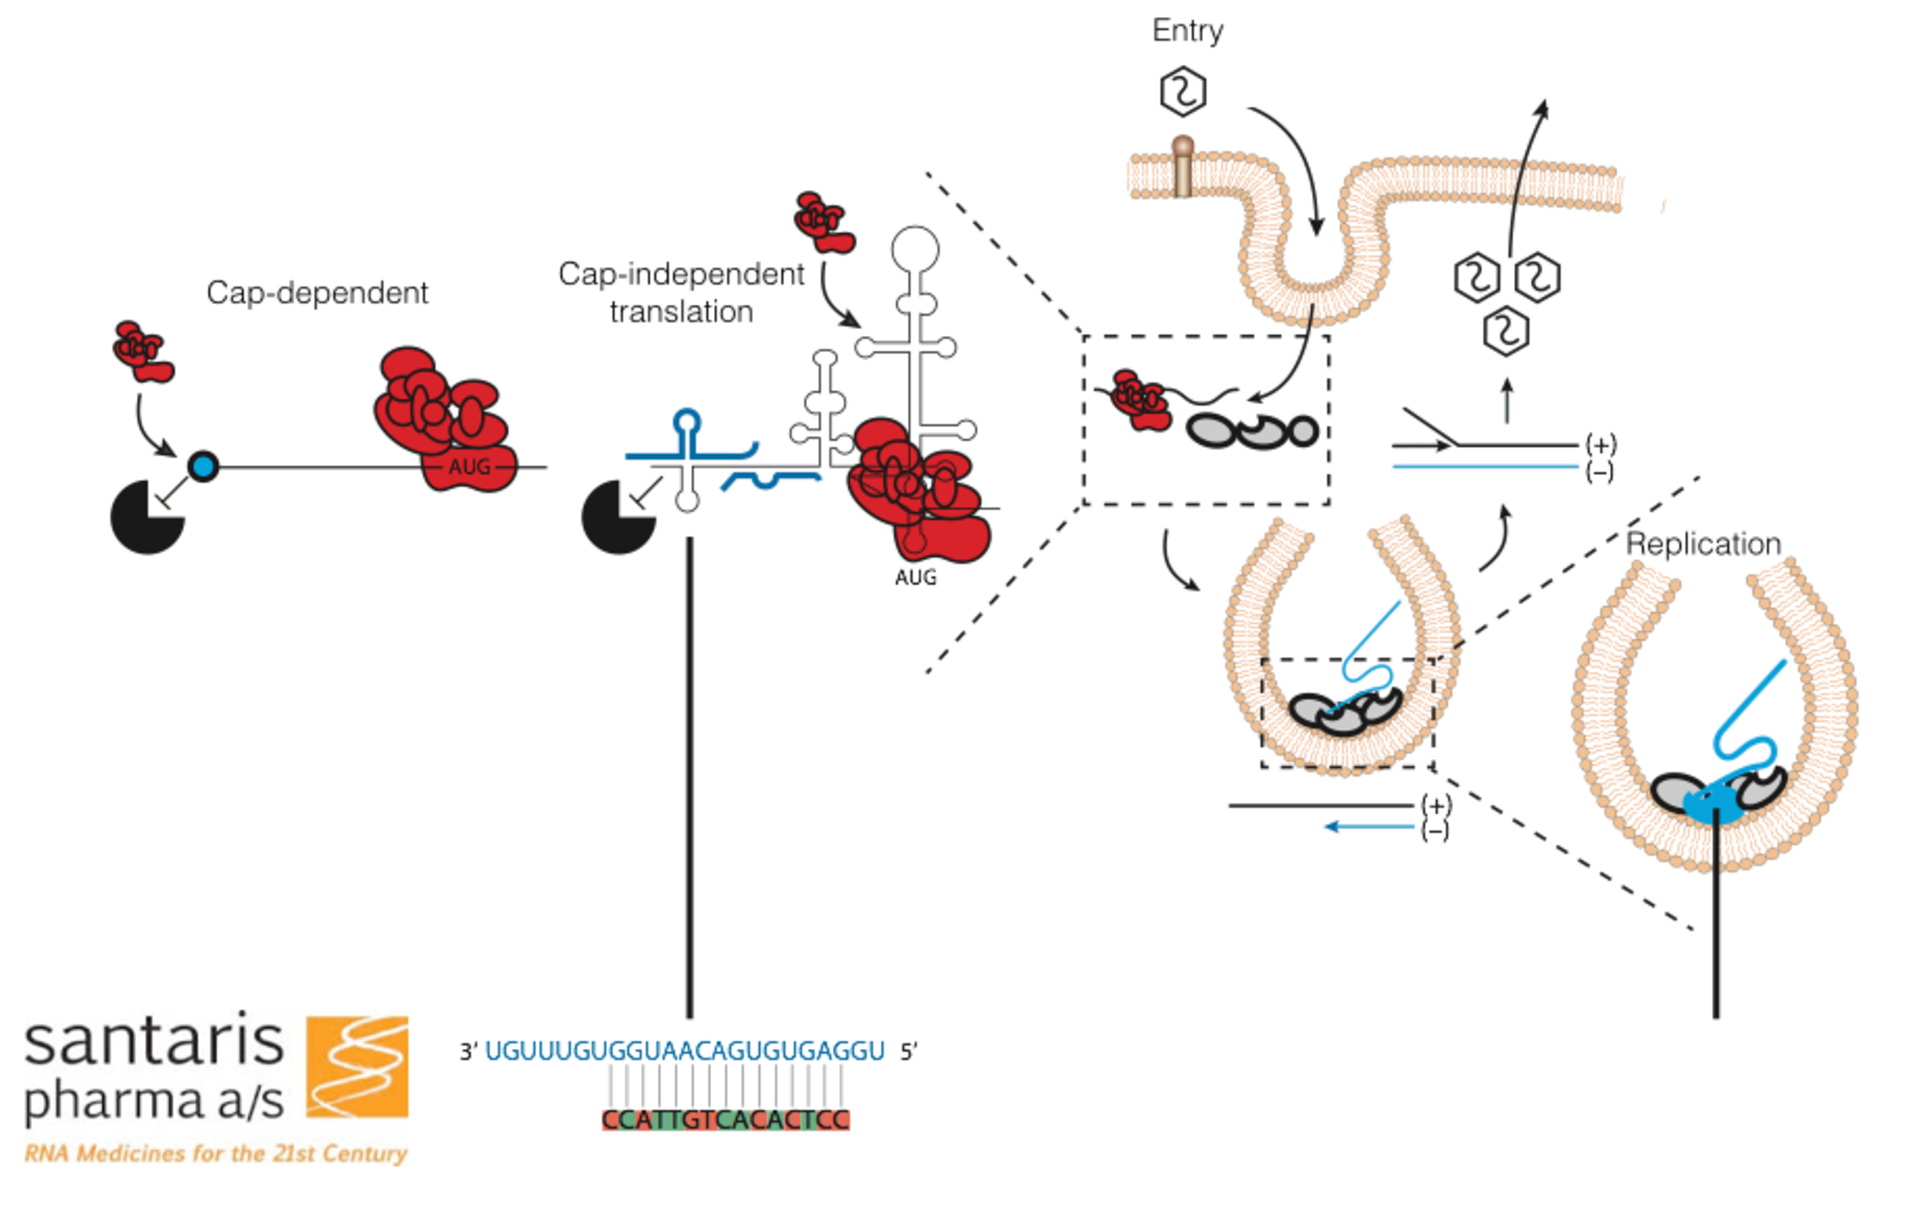
\includegraphics[width=140mm,scale=0.5]{Figures/Fig19}
\caption{Different modes of translation.}
\label{fig:Fig19}
\end{figure*}

Cellular mRNAs use cap-dependent translation, a process that involves interaction between initiation-factor proteins and the 7-methyl guanosine cap at the 5$'$ end of mRNA. This leads to 40S ribosome binding and scanning to the initiation codon, which is then followed by association with the 60S ribosomal subunit to form an active 80S ribosome that initiates translation of the protein (Figure ~\ref{fig:Fig19}).

An alternative pathway, called internal translation initiation, is a cap-independent mechanism of recruiting, positioning, and activating the eukaryotic protein-synthesis machinery driven by structured RNA sequences called internal ribosome entry sites (IRESs) that are located in the 5$'$ -untranslated region (UTR) of certain mRNAs \cite{Fraser:2006kn}. Lacking a 5$'$ cap, many RNA viruses contain IRES that mediate cap-independent translation. In this process, the virus commandeers cellular ribosomes as well as translation factors and signalling pathways that control the host protein synthesis. 

\section{HCV}

IRES-mediated translation is well-studied in the context of HCV and the structure of the 5$'$ UTR region is well-understood \cite{Fraser:2006kn}. Because of this, HCV is an excellent model system for extending the CLIP pipeline into infectious diseases. We approached this study by first identifying a protein that was (1) known to bind the HCV genome and (2) was critical for HCV replication, but (3) for which the mechanism of action remained unclear. We chose Poly-C binding protein 2 (PCBP2), a well-characterized RNA-binding protein with several studies linking it to HCV \cite{GarciaSastre:2013ko}.

\begin{figure*}
\center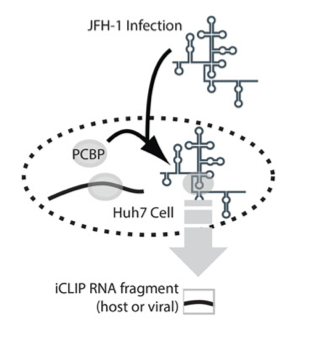
\includegraphics[width=80mm,scale=0.5]{Figures/Fig20}
\caption{CLIP applied to HCV virus.}
\label{fig:Fig20}
\end{figure*}

Though PCBP2 is required for HCV replication, the molecular details are poorly understood. Several studies focused on the HCV 5$'$ UTR have led to the suggestion that a complex between PCBP2 and SL1 of the 5$'$ UTR as well as an undefined region of the 3$'$ UTR of the viral RNA may be formed that facilitates viral circularization. Both SL1 and stem loop structures in the  3$'$ UTR of the viral genome are required for viral RNA replication. In addition, the proximity of SL1 to the conserved miR-122 sites in the HCV genome suggests that PCBP2 may coordinate with miR-122 in protection of the uncapped 5$'$ end of the viral RNA from degradation and/or the switch between viral translation and RNA replication \cite{GarciaSastre:2013ko}.


To elucidate the connection between PCBP2, translational regulation, and disease, we performed iCLIP in Huh-7 cells infected with the JFH-1 strain of Hepatitis C virus (HCV). We designed the pipeline so that it could easily be applied to viruses, and supplied the sequence of the JFH-1 genome as the mapping index (Figure ~\ref{fig:Fig20}). We generated coverage histograms of iCLIP RT stops across the HCV genome for two biological replicates, observing favorable concordance and global preference for binding U/C-rich regions of the genome ($r^2 = 0.93$) \cite{Flynn:2014bi}.

Consistent with prior studies, we observed a strong binding peak at SL1, but also detected PCBP2 occupancy that extends from SLI through the two miR-122 binding sites to the base of SL2. Surprisingly, we also detected strong binding around the translation start codon within SLVI of the internal ribosome entry site (IRES) (Figure ~\ref{fig:Fig21}). PCBP2$'$s interaction with viral 3$'$ UTR was significantly stronger than with the well-studied 5$'$ UTR. PCBP2 binding to the 3$'$ UTR occurred primarily in the single-stranded regions between stem-loops 5BSL3.2 and the variable region, a domain that includes the viral stop codon and that is implicated in both stimulation of translation and replication. Not surprisingly, PCBP2 also bound to the poly(U)/UC region of the viral genome, consistent with binding to single-stranded poly(U)/C regions. In addition to the UTRs, we observe multiple robust peaks of PCBP2 occupancy across the full viral gene body, which has never been reported.

\begin{figure*}
\center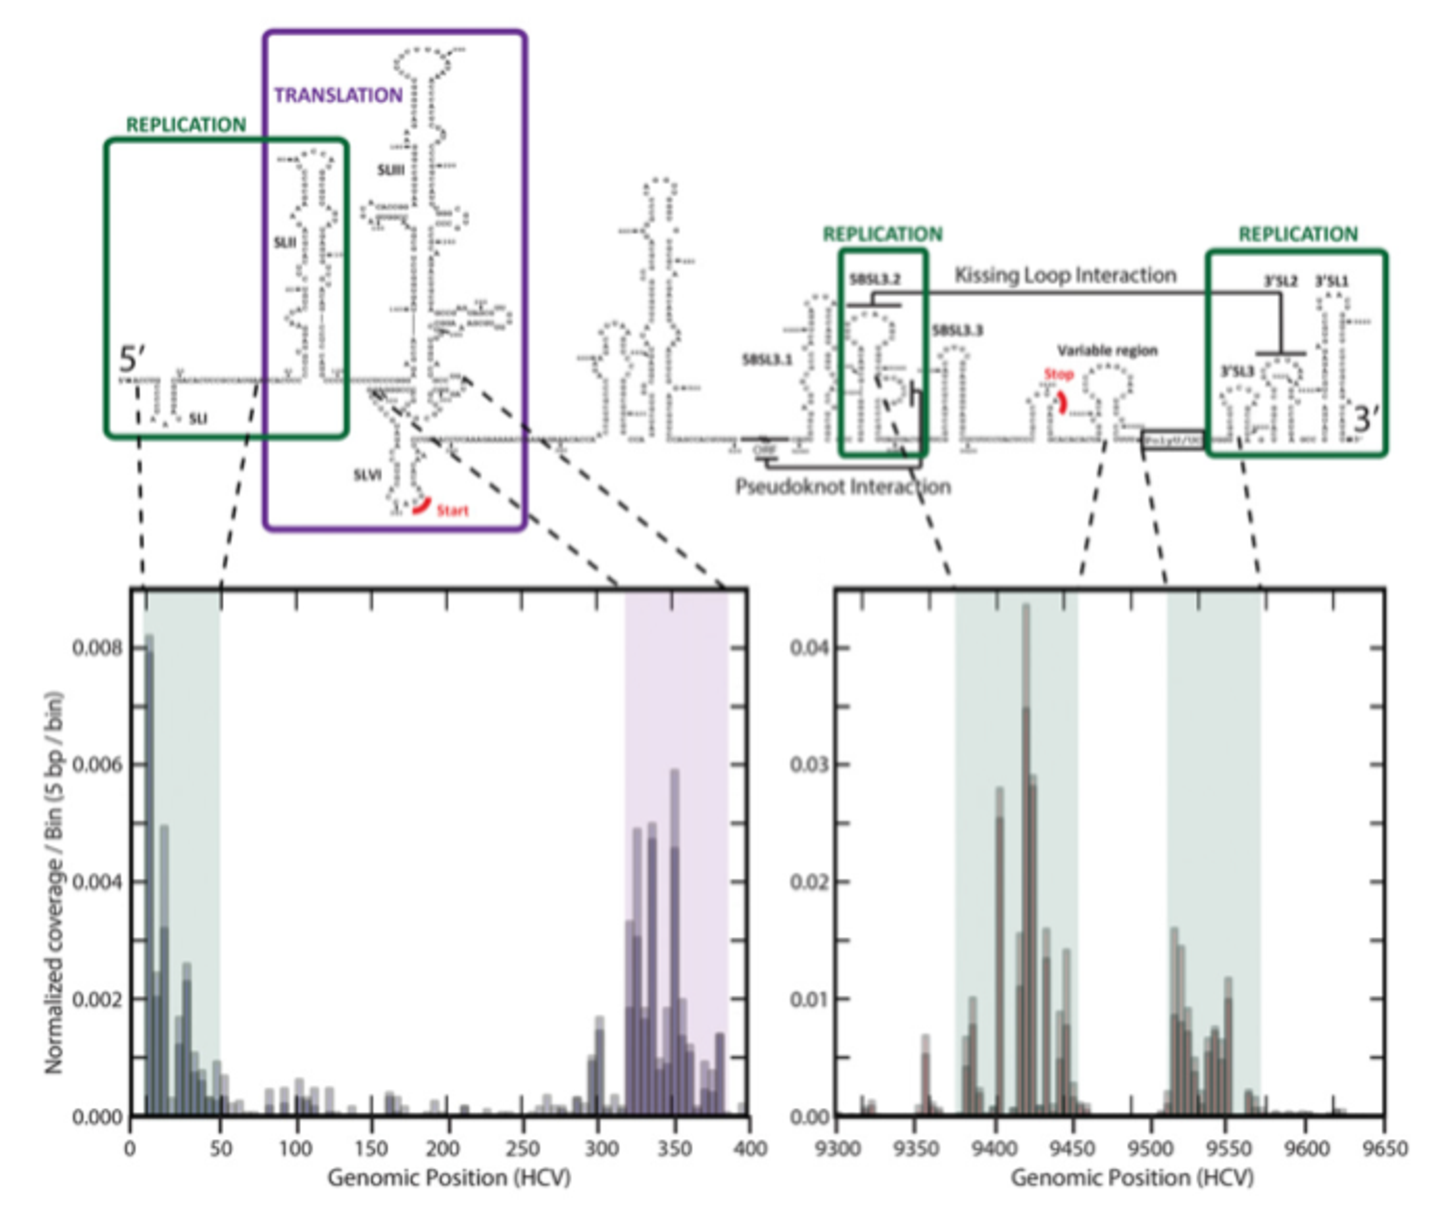
\includegraphics[width=150mm,scale=0.5]{Figures/Fig21}
\caption{PCBP binding profile on the HCV genome.}
\label{fig:Fig21}
\end{figure*}

Our application of FAST-iCLIP to HCV suggests that these regulatory functions of PCBP may be co-opted by the virus, as we also observe PCBP2 binding to the viral 5$'$ UTR, coding region, and 3$'$ UTR. We observe a peak of PCBP2 around the SL1/miR-122 binding site junction in the HCV genome, suggesting that PCBP2 may act in concert with miR-122 to restrict viral degradation from the 5$'$ UTR by cellular exonucleases such as Xrn2  \cite{GarciaSastre:2013ko}. PCBP2 also strongly bound to the translational start codon and the 3$'$ UTR of the HCV genome including the viral stop codon and conserved stem-loop structures required for viral RNA replication, a mode of binding that is topologically similar to that observed in poliovirus where it is well-known that PCBP2 plays a critical role in the viral life cycle \cite{Flynn:2014bi}.

\begin{figure*}
\center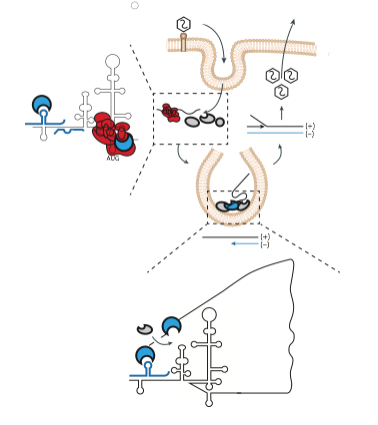
\includegraphics[width=100mm,scale=0.5]{Figures/Fig22}
\caption{Models for PCBP and HCV infection.}
\label{fig:Fig22}
\end{figure*}

In the context of a poliovirus infection, PCBP2 mediates cross-talk between the viral 5$'$ and 3$'$ UTRs in order to regulate the switch between viral translation and RNA replication. Our data are consistent with a symmetrical role for PCBP2 in the context of HCV infection and overlays in vivo biophysical detail from prior reports showing PCBP2-mediates circularization of the HCV genome \emph{in vitro}  \cite{Flynn:2014bi}. Thus, our application of FAST-iCLIP reveals a common binding topology of PCBP2 across the human transcriptome as well as the HCV genome. In both cases, a 3$'$ UTR bias is evident and suggests that PCBP2 regulatory functions may be co-opted by HCV.

\section{Retroviruses}

We have shown that CLIP can be 

Endogenous retroviruses 
~ 8% of genome
Normally silenced

HERV-K expressed in embryo:
After embryonic genome activation
During early blastocyst outgrowth

CLIP Rec, a viral protein
required for nuclear export in 
embryonic carcinoma cells (hECCs)

Read counts to regions in retroviral index  -

Hits in Rec-responsive element region -
Lower et. al. PNAS (1993, 1996)


(1) Export
(2) Protection against  exogenous infection (driving IFITM1)
(3) Engage cellular transcripts